\documentclass[14pt,aspectratio=169]{beamer}
%%%%%%%%%%%%%%%%%%%%%%%%%%%%%%%%%%%%%%%%%%%%%%%%%%%%%%%%%%%%%
% Meta informations:
\newcommand{\trauthor}{Imran Ibrahimli}
\newcommand{\trcourse}{Intelligent Adaptive Systems}
\newcommand{\trtitle}{Length Generalization on Multi-Digit Integer Addition with Transformers}
\newcommand{\trmatrikelnummer}{7486484}
\newcommand{\tremail}{imran.ibrahimli@studium.uni-hamburg.de}
\newcommand{\trinstitute}{Knowledge Technology, WTM \\ Dept. Informatik \\ Universit\"at Hamburg}
\newcommand{\trwebsiteordate}{{19.11.2024}}

%%%%%%%%%%%%%%%%%%%%%%%%%%%%%%%%%%%%%%%%%%%%%%%%%%%%%%%%%%%%%
% Languages:
\usepackage[english]{babel}
\selectlanguage{english}

%%%%%%%%%%%%%%%%%%%%%%%%%%%%%%%%%%%%%%%%%%%%%%%%%%%%%%%%%%%%%
% Bind packages:
\usepackage{beamerthemesplit}
\usetheme{Boadilla}
%\usetheme{Copenhagen}
%\usetheme{Darmstadt}
%\usetheme{Frankfurt}
%\usetheme{Ilmenau}
%\usetheme{JuanLesPins}
%\usetheme{Madrid}
%\usetheme{Warsaw }
%\usecolortheme{dolphin}
%\setbeamertemplate{sections/subsections in toc}[sections numbered]
%\beamertemplatenavigationsymbolsempty
%\setbeamertemplate{headline}[default] 	% deaktiviert die Kopfzeile
\setbeamertemplate{navigation symbols}{}% deaktiviert Navigationssymbole
%\useinnertheme{rounded}

\usepackage{acronym}                    % Acronyms
\usepackage{algorithmic}								% Algorithms and Pseudocode
\usepackage{algorithm}									% Algorithms and Pseudocode
\usepackage{amsfonts}                   % AMS Math Packet (Fonts)
\usepackage{amsmath}                    % AMS Math Packet
\usepackage{amssymb}                    % Additional mathematical symbols
\usepackage{amsthm}
\usepackage{color}                      % Enables defining of colors via \definecolor
\usepackage{fancybox}                   % Gleichungen einrahmen
\usepackage{fancyhdr}										% Paket zur schickeren der Gestaltung der 
\usepackage{graphicx}                   % Inclusion of graphics
%\usepackage{latexsym}                  % Special symbols
\usepackage{longtable}									% Allow tables over several parges
\usepackage{listings}                   % Nicer source code listings
\usepackage{lmodern}
\usepackage{multicol}										% Content of a table over several columns
\usepackage{multirow}										% Content of a table over several rows
\usepackage{rotating}										% Alows to rotate text and objects
\usepackage[section]{placeins}          % Ermoeglich \Floatbarrier fuer Gleitobj. 
\usepackage[hang]{subfigure}            % Allows to use multiple (partial) figures in a fig
%\usepackage[font=footnotesize,labelfont=rm]{subfig}	% Pictures in a floating environment
\usepackage{tabularx}										% Tables with fixed width but variable rows
\usepackage{booktabs}
\usepackage{url,xspace,boxedminipage}   % Accurate display of URLs


\definecolor{uhhRed}{RGB}{226,0,26}     % Official Uni Hamburg Red
\definecolor{uhhGrey}{RGB}{136,136,136} % Official Uni Hamburg Grey
\definecolor{uhhLightGrey}{RGB}{220, 220, 220}
\setbeamertemplate{itemize items}[ball]
\setbeamercolor{title}{fg=uhhRed,bg=white}
\setbeamercolor{title in head/foot}{bg=uhhRed}
\setbeamercolor{block title}{bg=uhhGrey,fg=white}
\setbeamercolor{block body}{bg=uhhLightGrey,fg=black}
\setbeamercolor{section in head/foot}{bg=black}
\setbeamercolor{frametitle}{bg=white,fg=uhhRed}
\setbeamercolor{author in head/foot}{bg=black,fg=white}
\setbeamercolor{author in footline}{bg=white,fg=black}
\setbeamercolor*{item}{fg=uhhRed}
\setbeamercolor*{section in toc}{fg=black}
\setbeamercolor*{separation line}{bg=black}
\setbeamerfont*{author in footline}{size=\scriptsize,series=\mdseries}
\setbeamerfont*{institute}{size=\footnotesize}

\newcommand{\opticalseperator}{0.0025\paperwidth}

\institute{Universit\"at Hamburg\\\trinstitute}
\title{\trtitle}
\author{\trauthor}
\date{}
\logo{}

%%%%%%%%%%%%%%%%%%%%%%%%%%%%%%%%%%%%%%%%%%%%%%%%%%%%%%%%%%%%%
% Configurationen:
%\hypersetup{pdfpagemode=FullScreen}

\hyphenation{whe-ther} 									% Manually use: "\-" in a word: Staats\-ver\-trag

%\lstloadlanguages{C}                   % Set the default language for listings
\DeclareGraphicsExtensions{.pdf,.svg,.jpg,.png,.eps} % first try pdf, then eps, png and jpg
\graphicspath{{./img/}} 								% Path to a folder where all pictures are located

%%%%%%%%%%%%%%%%%%%%%%%%%%%%
% Costom Definitions:
\setbeamertemplate{title page}
{
    \vspace{0.4cm}
    \begin{centering}
        % Title at the top
        \begin{beamercolorbox}[sep=8pt,center,colsep=-4bp]{title}
            \usebeamerfont{title}\inserttitle\par%
            \ifx\insertsubtitle\@empty%
            \else%
                \vskip0.20em%
                {\usebeamerfont{subtitle}\usebeamercolor[fg]{subtitle}\insertsubtitle\par}%
            \fi%
        \end{beamercolorbox}%
        \vskip0.4em
    \end{centering}

    % Content below the title: side-by-side layout
    \begin{columns}[c]
        % Left column for author info and advisors
        \hskip0.05\textwidth
        \begin{column}{0.7\textwidth}
            \begin{beamercolorbox}[sep=8pt,center,colsep=-4bp,rounded=true,shadow=true]{author}
                \raggedright
                \usebeamerfont{author}\insertauthor \\ 
                \texttt{\tremail} \\ 
                \trinstitute
            \end{beamercolorbox}
            \vskip0.2em
            \begin{beamercolorbox}[sep=8pt,center,colsep=-4bp,rounded=true,shadow=true]{advisors}
                \raggedright
                \usebeamerfont{author}Advisors: \\ Prof. Dr. Stefan Wermter, Dr. Jae Hee Lee
            \end{beamercolorbox}
        \end{column}

        % Right column for the logo
        \begin{column}{0.3\textwidth}
            \vfill
            \raggedleft
            
\includegraphics[width=0.7\textwidth]{wtmIcon.pdf}
            \vfill
        \end{column}
        \hskip0.05\textwidth

    \end{columns}

    % Footer (optional)
    \vfill
    \begin{beamercolorbox}[sep=8pt,center,colsep=-4bp,rounded=true,shadow=true]{institute}
    \usebeamerfont{institute}\trwebsiteordate
    \end{beamercolorbox}
    \vspace{-0.1cm}
}


\setbeamertemplate{frametitle}
{
\begin{beamercolorbox}[wd=\paperwidth,ht=3.8ex,dp=1.2ex,leftskip=0pt,rightskip=4.0ex]{frametitle}%
		\usebeamerfont*{frametitle}\centerline{\insertframetitle}
	\end{beamercolorbox}
	\vspace{0.0cm}
}

\setbeamertemplate{footline}
{
  \leavevmode
	\vspace{-0.05cm}
  \hbox{
	  \begin{beamercolorbox}[wd=.32\paperwidth,ht=4.8ex,dp=2.7ex,center]{author in footline}
	    \hspace*{2ex}\usebeamerfont*{author in footline}\trauthor
	  \end{beamercolorbox}%
	  \begin{beamercolorbox}[wd=.60\paperwidth,ht=4.8ex,dp=2.7ex,center]{author in footline}
	    \usebeamerfont*{author in footline}\trtitle
	  \end{beamercolorbox}%
	  \begin{beamercolorbox}[wd=.07\paperwidth,ht=4.8ex,dp=2.7ex,center]{author in footline}
	    \usebeamerfont*{author in footline}\insertframenumber{}
	  \end{beamercolorbox}
  }
	\vspace{0.15cm}
}
\renewcommand{\footnotesize}{\fontsize{12.4pt}{12.4pt}\selectfont}
\renewcommand{\small}{\fontsize{13.8pt}{13.8pt}\selectfont}
\renewcommand{\normalsize}{\fontsize{15.15pt}{15.15pt}\selectfont}
\renewcommand{\large}{\fontsize{17.7pt}{17.7pt}\selectfont}
\renewcommand{\Large}{\fontsize{21.3pt}{21.3pt}\selectfont}

%%%%%%%%%%%%%%%%%%%%%%%%%%%%
% Additional 'theorem' and 'definition' blocks:
\newtheorem{axiom}{Axiom}[section] 	
%\newtheorem{axiom}{Fakt}[section]			% Wenn in Deutsch geschrieben wird.
%Usage:%\begin{axiom}[optional description]%Main part%\end{fakt}

%Additional types of axioms:
\newtheorem{observation}[axiom]{Observation}

%Additional types of definitions:
\theoremstyle{remark}
%\newtheorem{remark}[section]{Bemerkung} % Wenn in Deutsch geschrieben wird.
\newtheorem{remark}[section]{Remark} 

%%%%%%%%%%%%%%%%%%%%%%%%%%%%
% Provides TODOs within the margin:
\newcommand{\TODO}[1]{\marginpar{\emph{\small{{\bf TODO: } #1}}}}

%%%%%%%%%%%%%%%%%%%%%%%%%%%%
% Abbreviations and mathematical symbols
\newcommand{\modd}{\text{ mod }}
\newcommand{\RS}{\mathbb{R}}
\newcommand{\NS}{\mathbb{N}}
\newcommand{\ZS}{\mathbb{Z}}
\newcommand{\dnormal}{\mathit{N}}
\newcommand{\duniform}{\mathit{U}}

\newcommand{\erdos}{Erd\H{o}s}
\newcommand{\renyi}{-R\'{e}nyi}

%%%%%%%%%%%%%%%%%%%%%%%%%%%%
% Display of TOCs:
\AtBeginSection[]
{
	\setcounter{tocdepth}{2}  
	\frame
	{
	  \frametitle{Outline}
		\tableofcontents[currentsection]
	}
}
 

%%%%%%%%%%%%%%%%%%%%%%%%%%%%%%%%%%%%%%%%%%%%%%%%%%%%%%%%%%%%%
% Document:
\begin{document}

\begin{frame}[plain]
    \titlepage
\end{frame}

\frame{
    \frametitle{Outline}
    \tableofcontents
}

\section{Introduction}

\begin{frame}
    \frametitle{Motivation}
    \begin{itemize}
        \item Transformer models are being adopted across many domains from language modeling to robotics.
        \item For effective applications, models need to learn generalizing operations or algorithms from data.
        \item Generalization enhances robustness and trust in AI systems.
    \end{itemize}
\end{frame}

\begin{frame}
    \frametitle{Motivation (cont.)}
    \begin{itemize}
        \item Examine a simple toy task: integer addition.
        \item We don't need transformers to perform addition.
        \item But we care if they can learn ``simple'' algorithms from examples.
        \item Length-generalizable multi-digit addition is an open problem for transformers.
        \item Actively worked on with many papers in NeurIPS, ICLR, etc.
    \end{itemize}
\end{frame}

\begin{frame}
    \frametitle{Motivation (cont.)}
    \begin{itemize}
        \item Example: even SOTA model GPT-4o struggles with addition.
    \end{itemize}
    \begin{figure}
        \centering
        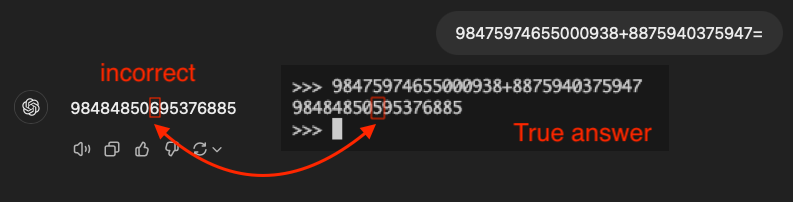
\includegraphics[width=0.9\textwidth]{fig/gpt4o_add_fail.png}
    \end{figure}
\end{frame}

\begin{frame}
    \frametitle{Motivation (cont.)}
    \begin{itemize}
        \item Why is this important?
        \item Maybe just guardrail models by hard-coding some rules?
        \item Not generally, because we would not train and use the models, if we could hard-code the rules in the first place.
        \item We want to understand the limitations of the models and improve them.
    \end{itemize}
\end{frame}

\begin{frame}
    \frametitle{Problem Statement}
    \begin{itemize}
        \item Focus on standard decoder-only transformers with absolute positional encodings.
        \item Try to improve generalization without altering model architecture or task-specific modifications.
        \item Explore data formatting and training data diversity.
    \end{itemize}
\end{frame}

\begin{frame}
    \frametitle{Research Questions}
    \begin{enumerate}
        \item Why do transformers with absolute positional encodings fail to generalize integer addition to longer sequences?
        \item How does the inclusion of sub-task data influence the model's compositionality and length generalization capabilities?
    \end{enumerate}
\end{frame}

\section{Background}

\begin{frame}
    \frametitle{Transformers}
    \begin{columns}
        \begin{column}{0.6\textwidth}
            \begin{itemize}
                \item Utilize self-attention to process sequential data.
                \item Focus on decoder-only models (b).
                \item Capable of capturing long-range dependencies without recurrence.
            \end{itemize}
        \end{column}
        \begin{column}{0.4\textwidth}
            \begin{figure}
                \centering
                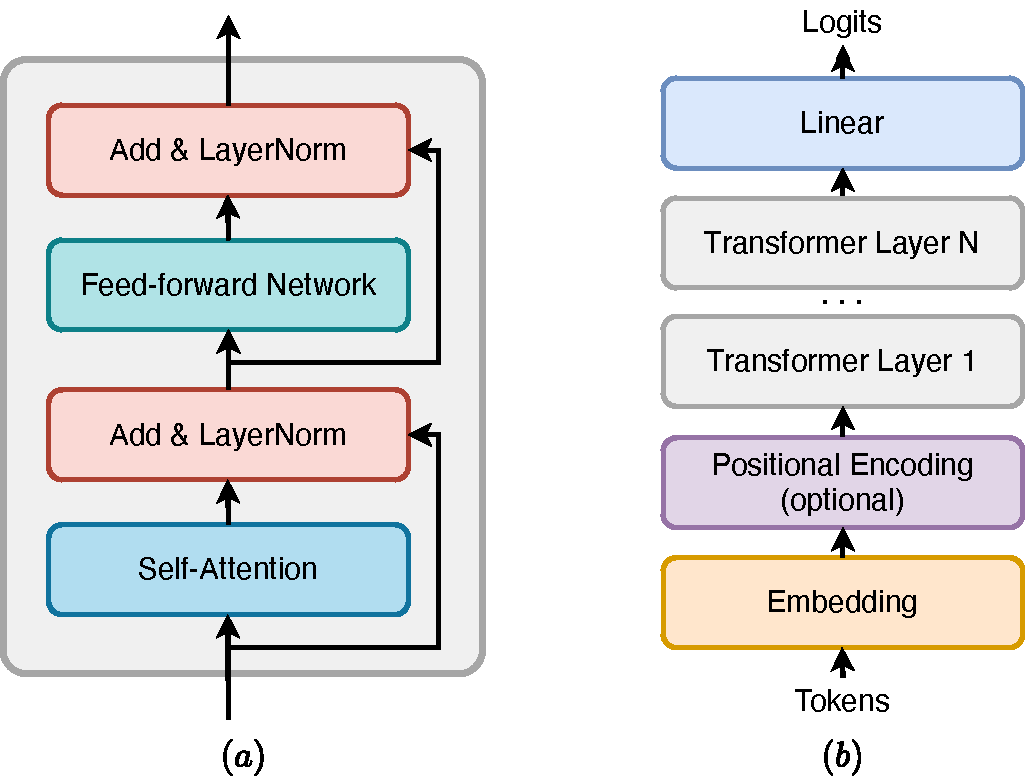
\includegraphics[width=\textwidth]{fig/transformer_layer.pdf}
            \end{figure}
        \end{column}
    \end{columns}
\end{frame}

\begin{frame}
    \frametitle{Positional Encodings (PE)}
    \begin{itemize}
        \item No explicit positional awareness in transformers.
        \item PEs inject sequence order information.
        \item Can be absolute or relative.
              \begin{itemize}
                  \item Absolute PEs: \\ \texttt{0, 1, 2, 3, ...}
                  \item Relative PEs: \\ \texttt{..., -3, -2, -1, 0, 1, 2, 3, ...}
              \end{itemize}
    \end{itemize}
\end{frame}

\begin{frame}
    \frametitle{Absolute Positional Encoding}
    \begin{itemize}
        \item Adds fixed positional information to input embeddings.
        \item Sinusoidal absolute PEs introduced by Vaswani et al. (2017):
              \[
                  \begin{aligned}
                      \text{PE}_{(pos, 2i)}   & = \sin\left( \frac{pos}{10000^{2i / d_{\text{model}}}} \right) \\
                      \text{PE}_{(pos, 2i+1)} & = \cos\left( \frac{pos}{10000^{2i / d_{\text{model}}}} \right)
                  \end{aligned}
              \]
    \end{itemize}
\end{frame}

\section{Related Work}
\begin{frame}
    \frametitle{Challenges in Length Generalization}
    \begin{itemize}
        \item Positional encoding plays a significant role.
        \item Kazemnejad et al. (2023) find even models without positional encodings can length generalize somewhat.
        \item Experiments in this thesis do not support these findings.
    \end{itemize}
\end{frame}

\begin{frame}
    \frametitle{Issues with Positional Encodings}
    \begin{itemize}
        \item Models struggle to select relevant tokens based on position in longer sequences.
        \item Failure to \textbf{align digits} without explicit positional cues.
        \item Confirmed by multiple studies (Shen et al. 2023; Zhao et al. 2024).
    \end{itemize}
\end{frame}

\begin{frame}
    \frametitle{Improving Length Generalization}
    \begin{itemize}
        \item Reversing answer and training with scratchpad (Lee et al. 2024).
        \item Randomized PEs (Ruoss et al. 2023).
        \item Inclusion of random spaces in input (Shen et al. 2023).
        \item Index hints \texttt{a1b2c3+a4b5c6=a5b7c9} (Y. Zhou et al. 2024)
        \item Task-specific PEs, e.g. Abacus (McLeish et al. 2024).
    \end{itemize}
\end{frame}

\begin{frame}
    \frametitle{Length Generalization Ratio}
    \begin{itemize}
        \item Ratio of the length of solved test problems to training lengths.
        \item 1.1x ratio achieved by Shen et al. (2023).
        \item 1.125x by Kazemnejad et al. (2023).
        \item 1.5x by H. Zhou et al. (2023).
        \item 2.5x with FIRE and index hints (Y. Zhou et al. 2024).
        \item \textbf{6x} achieved with Abacus encoding (McLeish et al. 2024).
    \end{itemize}
\end{frame}

\begin{frame}
    \frametitle{Abacus Encoding}
    \begin{itemize}
        \item Encode digit position relative to the start of the number.
        \item Need to reverse integers
        \item Use sinusoidal PE with indices specified by the Abacus encoding.
        \item Combined with architectural modifications like input injection and recurrent layers.
        \item Trained on up to 20 digits, generalizes to 120 digits.
    \end{itemize}
    \begin{figure}
        \centering
        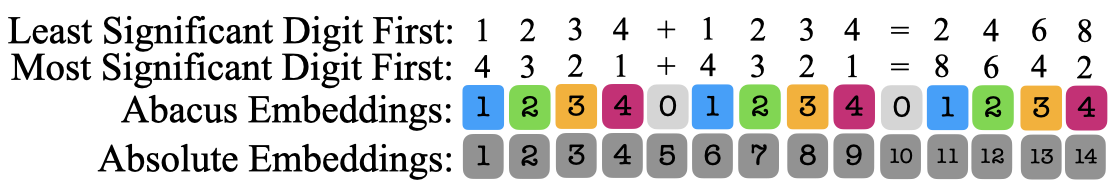
\includegraphics[width=0.7\textwidth]{fig/abacus.png}
        \caption{Source: McLeish et al. (2024)}
    \end{figure}
\end{frame}

\begin{frame}
    \frametitle{Conclusions from Related Work}
    \begin{itemize}
        \item No common benchmark $\rightarrow$ hard to compare methods.
        \item Positional encodings and data formatting significantly impact length generalization.
        \item Task-specific design can boost generalization to unseen lengths.
        \item Some diverge from standard decoder unsupervised training.
    \end{itemize}
\end{frame}

\begin{frame}
    \frametitle{Limitations of Existing Methods}
    \begin{itemize}
        \item Some successful methods lose sight of the original task:\\
              It's not about addition, but about model capabilities.
        \item Task-specific modifications are not always feasible.
        \item For the same reason e.g. adding index hints is "hacky."
        \item Desire for simpler methods without altering model architecture.
    \end{itemize}
\end{frame}

\section{Approach}

\begin{frame}
    \frametitle{Overview of Approach}
    \begin{itemize}
        \item Investigate various positional encodings and data formatting.
        \item Examine the impact of sub-task data on compositionality.
        \item Apply mechanistic interpretability to analyze models.
    \end{itemize}
\end{frame}

\begin{frame}
    \frametitle{Data Formatting Techniques}
    \begin{table}
        \centering
        \begin{tabular}{ll}
            \toprule
            Technique         & Example                     \\
            \midrule
            Standard format   & \texttt{123+456=}           \\
            Reversed operands & \texttt{321+654=}           \\
            Random spaces     & \texttt{1 23 +4  5 6=}      \\
            Zero-padding      & \texttt{00123+00456=}       \\
            Scratchpad        & \texttt{\$567+789=765+987;} \\
                              & \texttt{c=0,7+0+0=7,c=0;}   \\
                              & \texttt{6+9+0=5,c=1;}       \\
                              & \texttt{5+8+1=4,c=1;}       \\
                              & \texttt{0+7+1=8,c=0|8457\$} \\
            \bottomrule
        \end{tabular}
    \end{table}
\end{frame}

\begin{frame}
    \frametitle{Reproducing Baseline Failure: Results}
    \begin{itemize}
        \item High accuracy on training lengths (1 and 3 digits).
        \item Significant drop in accuracy on unseen lengths (2 and 4 digits).
    \end{itemize}
    \begin{figure}
        \centering
        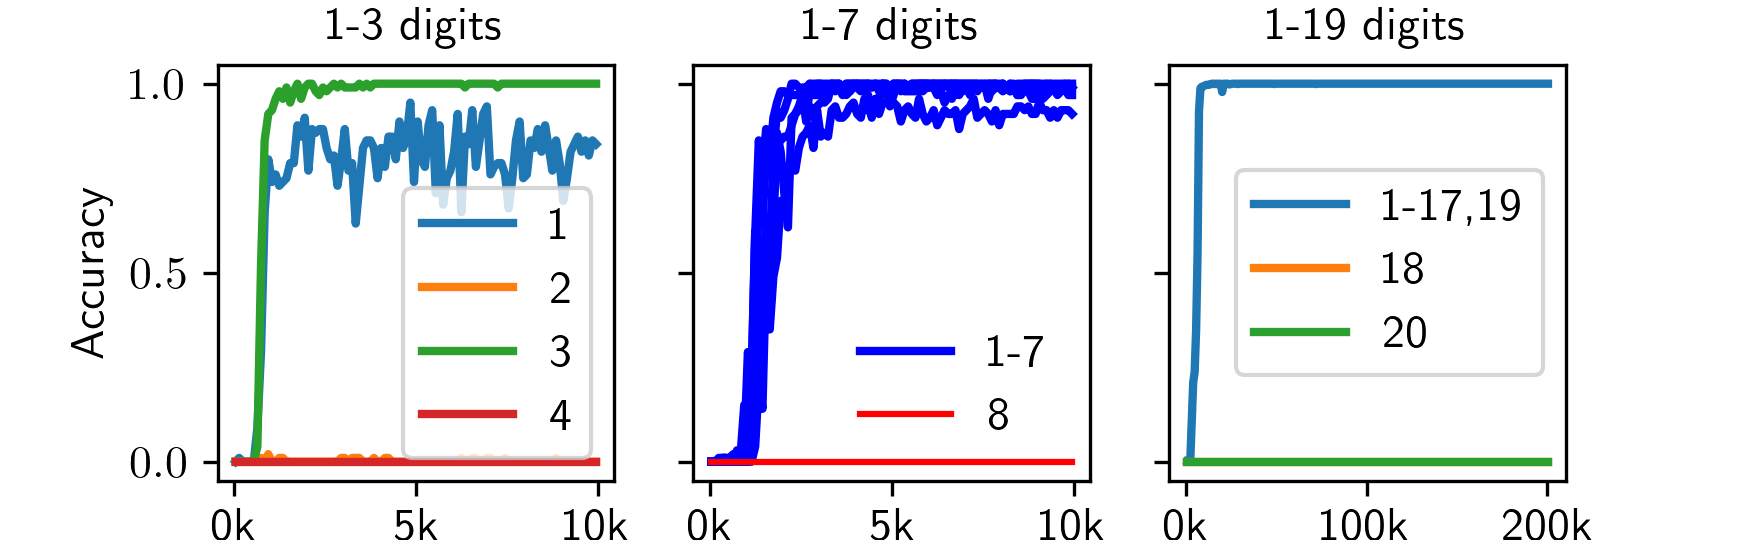
\includegraphics[width=0.8\textwidth]{fig/baseline_and_longer.png}
        \caption{Baseline performance over training epochs.}
    \end{figure}
\end{frame}

\begin{frame}
    \frametitle{Reproducing Baseline Failure: Analysis}
    \begin{itemize}
        \item Model relies on absolute positions seen during training.
        \item Fails to align digits correctly for unseen lengths.
        \item Highlights limitations of absolute positional encoding.
    \end{itemize}
\end{frame}

\begin{frame}
    \frametitle{Extending Baseline Observations}
    \begin{itemize}
        \item Trained on 1-7 digit additions.
        \item Tested on 8-digit additions.
        \item Consistent failure to generalize to longer sequences.
    \end{itemize}
\end{frame}

\begin{frame}
    \frametitle{Assessing Generalization Across Lengths}
    \begin{itemize}
        \item Trained on 1-19 digit additions (excluding 18-digit cases).
        \item Tested on 1-20 digit additions.
        \item No significant generalization to unseen lengths.
    \end{itemize}
\end{frame}

\begin{frame}
    \frametitle{Impact of Data Formatting and Dataset Size}
    \begin{itemize}
        \item Introduced random spaces in input sequences.
        \item Trained on 1-7 and 9-digit additions.
        \item Tested on 8 and 10-13 digits.
        \item Slight improvement in length generalization observed.
    \end{itemize}
    \begin{figure}
        \centering
        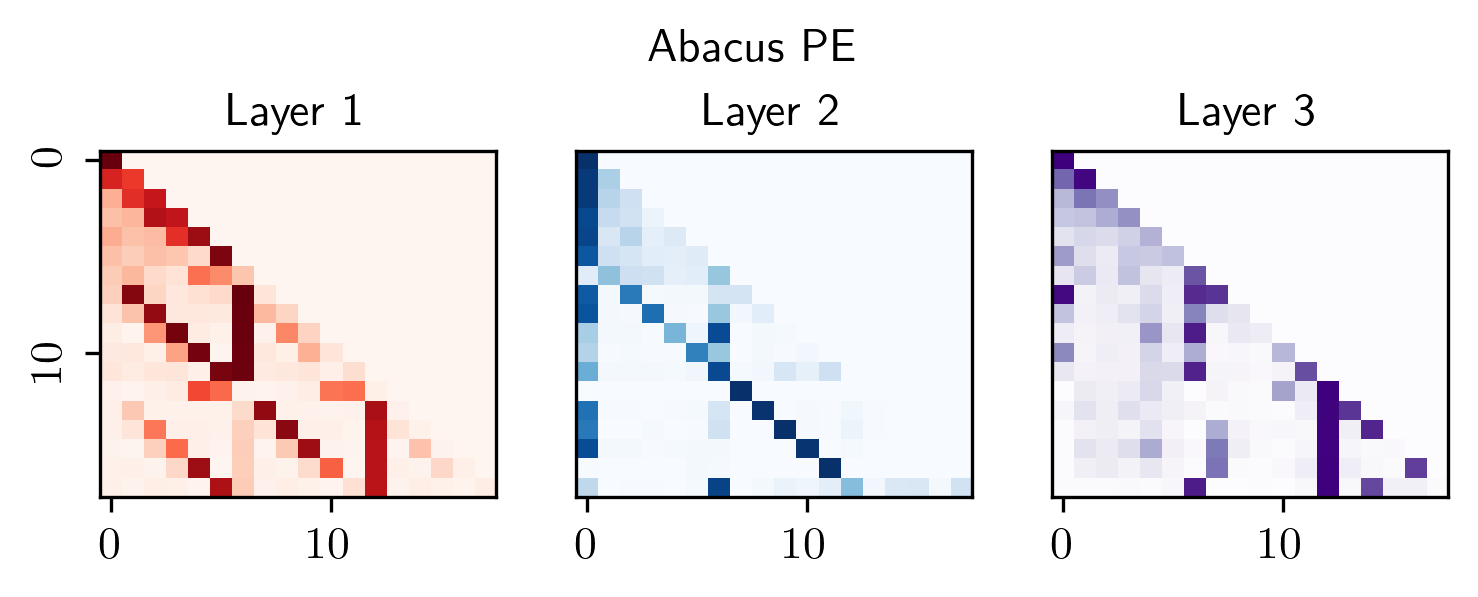
\includegraphics[width=0.8\textwidth]{fig/attn_map_abacus_pe.png}
        \caption{Attention maps with random spaces in input sequences.}
    \end{figure}
\end{frame}

\begin{frame}
    \frametitle{Introducing Sub-Task Data}
    \begin{itemize}
        \item Sub-tasks: carry detection, modular addition, reversing, digit alignment.
        \item Used task-specific prefixes to distinguish tasks.
        \item Trained models on combined data.
    \end{itemize}
    \begin{table}
        \centering
        \caption{Examples of Sub-Task Data}
        \begin{tabular}{ll}
            \toprule
            Sub-Task         & Example                       \\
            \midrule
            Modular Addition & \texttt{mod\_add: 7 + 8 = 5}  \\
            Carry Detection  & \texttt{carry: 7 + 8 = 1}     \\
            Reversing        & \texttt{reverse: 123 = 321}   \\
            Digit Alignment  & \texttt{align:  123}          \\
                             & \hspace{1.2cm} \texttt{+ 456} \\
            \bottomrule
        \end{tabular}
    \end{table}
\end{frame}

\begin{frame}
    \frametitle{Effect on Compositionality}
    \begin{itemize}
        \item Analyzed the model's ability to compose functions.
        \item Marginal improvements in length generalization observed.
        \item Smaller models benefited more from sub-task training.
    \end{itemize}
    \begin{figure}
        \centering
        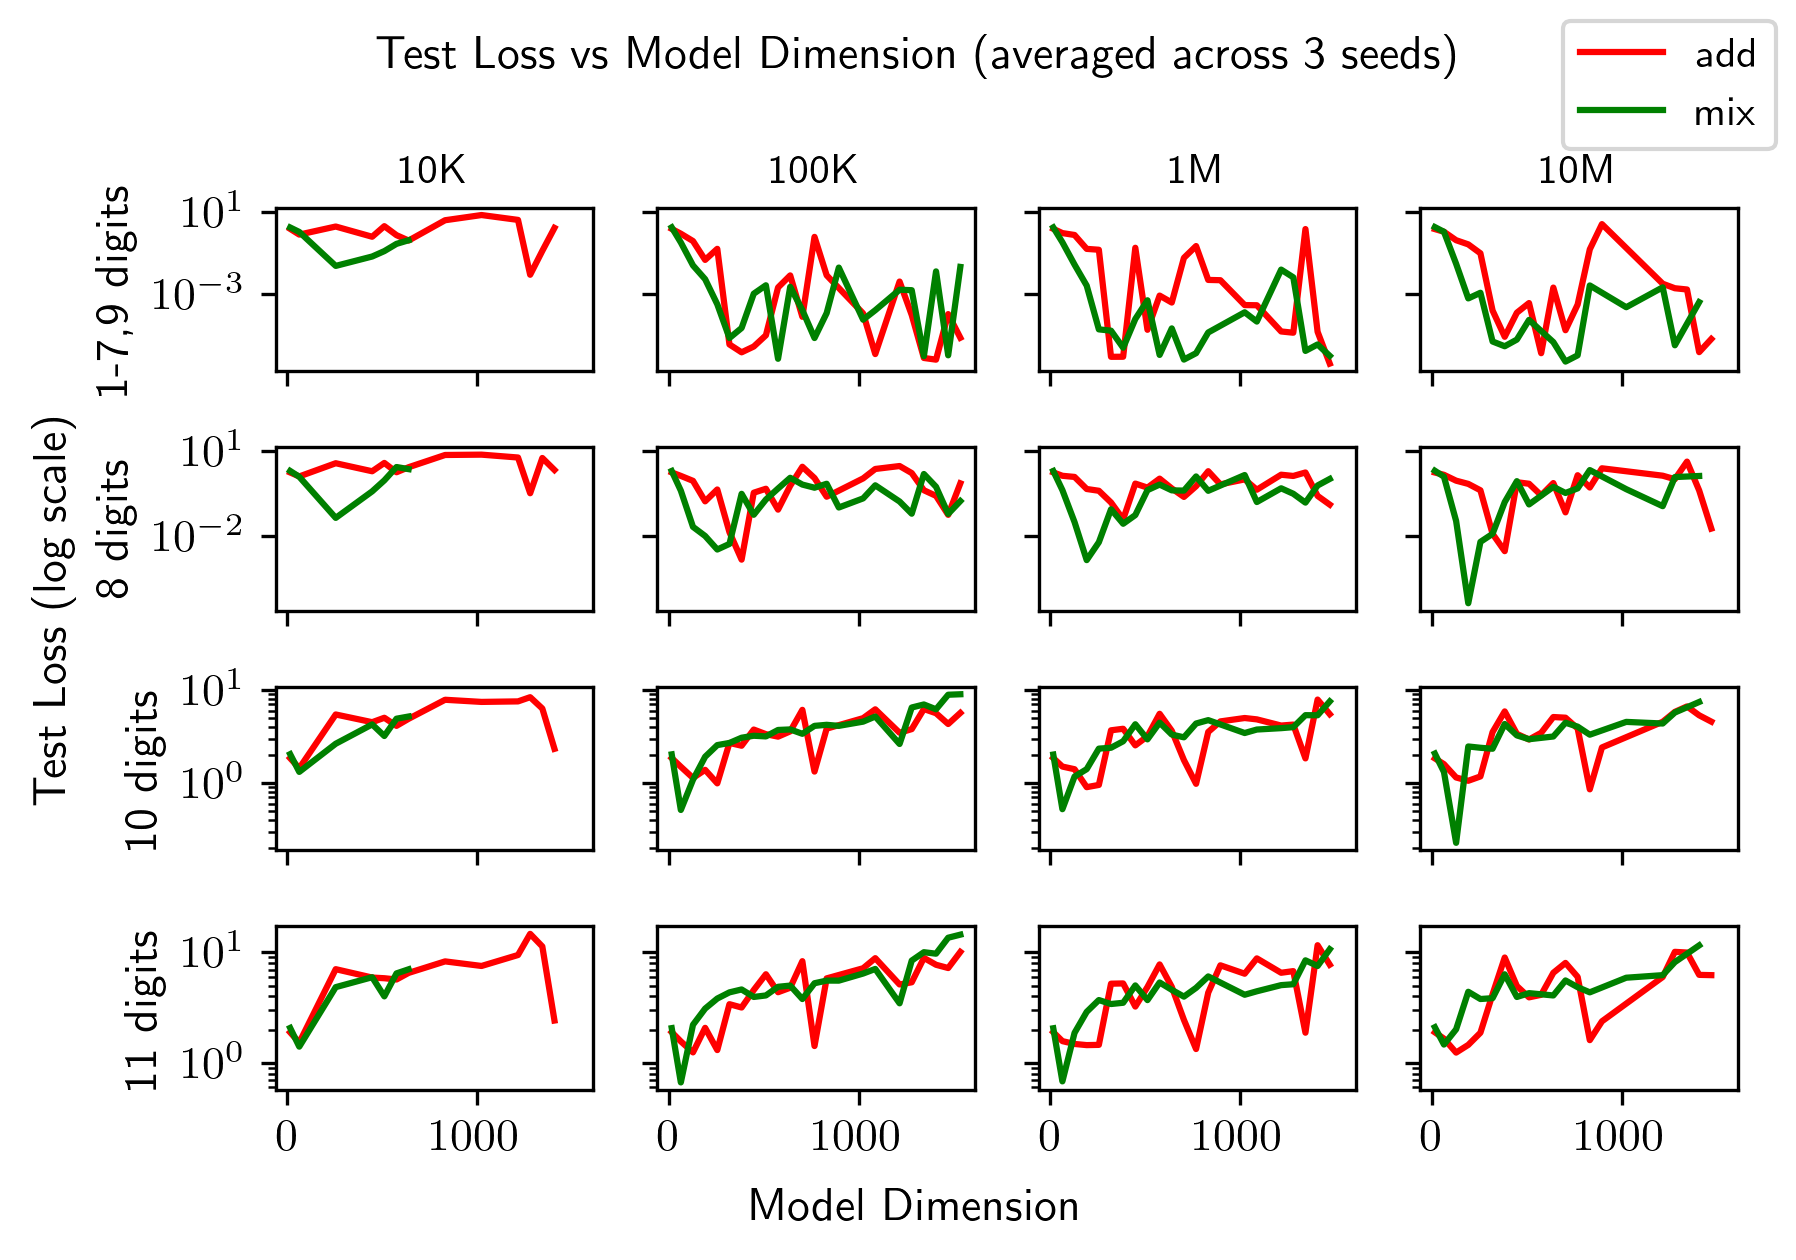
\includegraphics[width=0.8\textwidth]{fig/exp_27_val_loss_vs_n_embd.png}
        \caption{Test loss vs. model dimension for addition-only and multi-task training.}
    \end{figure}
\end{frame}

\begin{frame}
    \frametitle{Comprehensive Analysis Across Scales}
    \begin{itemize}
        \item Explored model dimensions from 64 to 1536.
        \item Dataset sizes from 10K to 10M examples.
        \item Compared models trained with and without sub-task data.
    \end{itemize}
\end{frame}

\begin{frame}
    \frametitle{Sub-Task Difficulty Analysis}
    \begin{itemize}
        \item Evaluated test loss and accuracy for sub-tasks.
        \item Modular addition and digit alignment were most challenging.
        \item Significant variability in performance across sub-tasks.
    \end{itemize}
    \begin{figure}
        \centering
        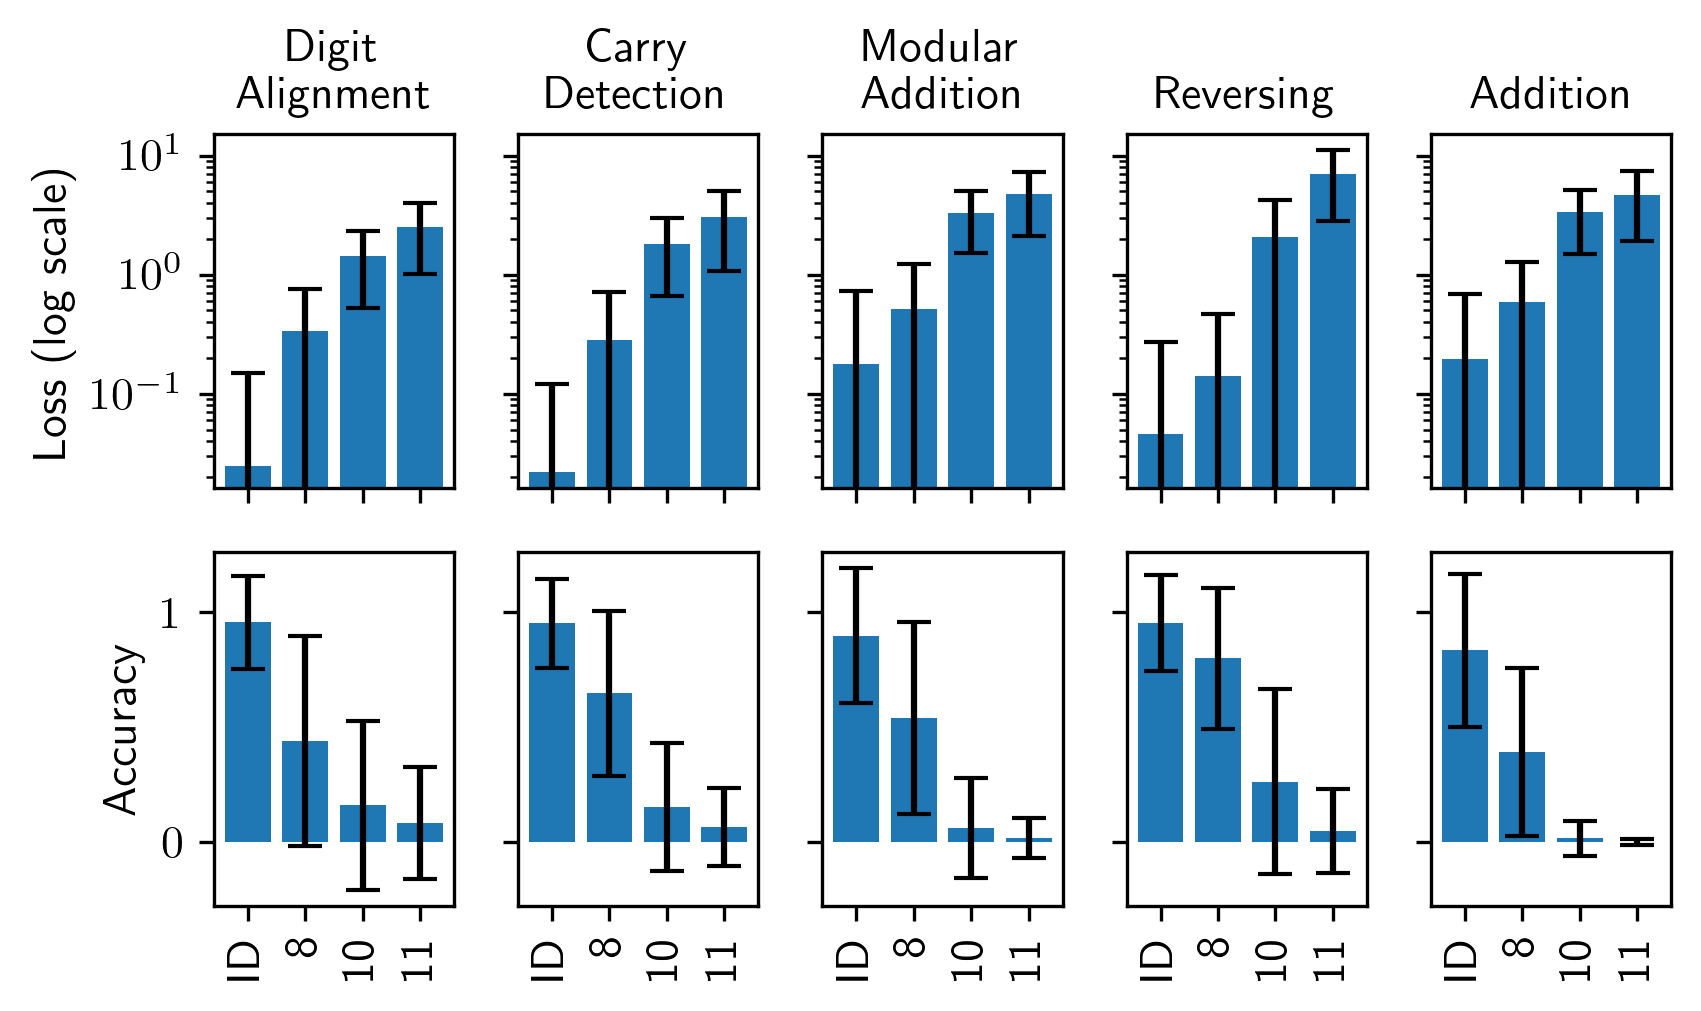
\includegraphics[width=0.8\textwidth]{fig/subtask_difficulty.png}
        \caption{Sub-task difficulty analysis.}
    \end{figure}
\end{frame}

\begin{frame}
    \frametitle{Mechanistic Interpretability}
    \begin{itemize}
        \item Analyzed attention maps of models.
        \item Models with Abacus encoding showed crisp attention patterns.
        \item Models with absolute positional encoding had diffuse attention.
        \item Indicates challenges in digit alignment and carry propagation.
    \end{itemize}
\end{frame}

\section{Conclusion}

\begin{frame}
    \frametitle{Summary of Findings}
    \begin{itemize}
        \item Transformer models with absolute positional encodings fail to generalize due to rigid digit alignment.
        \item Abacus positional encoding significantly improves length generalization.
        \item Data formatting techniques offer marginal improvements.
        \item Sub-task data enhances compositionality, especially in smaller models.
        \item Mechanistic interpretability reveals differences in internal representations.
    \end{itemize}
\end{frame}

\begin{frame}
    \frametitle{Future Work}
    \begin{itemize}
        \item Develop positional encodings that generalize without task-specific modifications.
        \item Explore other data augmentation techniques to improve generalization.
        \item Apply mechanistic interpretability to more complex tasks.
        \item Investigate the impact of model architecture variations on length generalization.
    \end{itemize}
\end{frame}

\begin{frame}
    \frametitle{Questions}
    \centering
    Thank you for your attention! \\
    \vspace{1cm}
    Questions?
\end{frame}


% Appendix

\begin{frame}
    \frametitle{Appendix: Counting Failure}
    \begin{itemize}
        \item Example: SOTA model GPT-4o struggles with simple counting.
    \end{itemize}
    \begin{figure}
        \centering
        \begin{minipage}{0.55\textwidth}
            \centering
            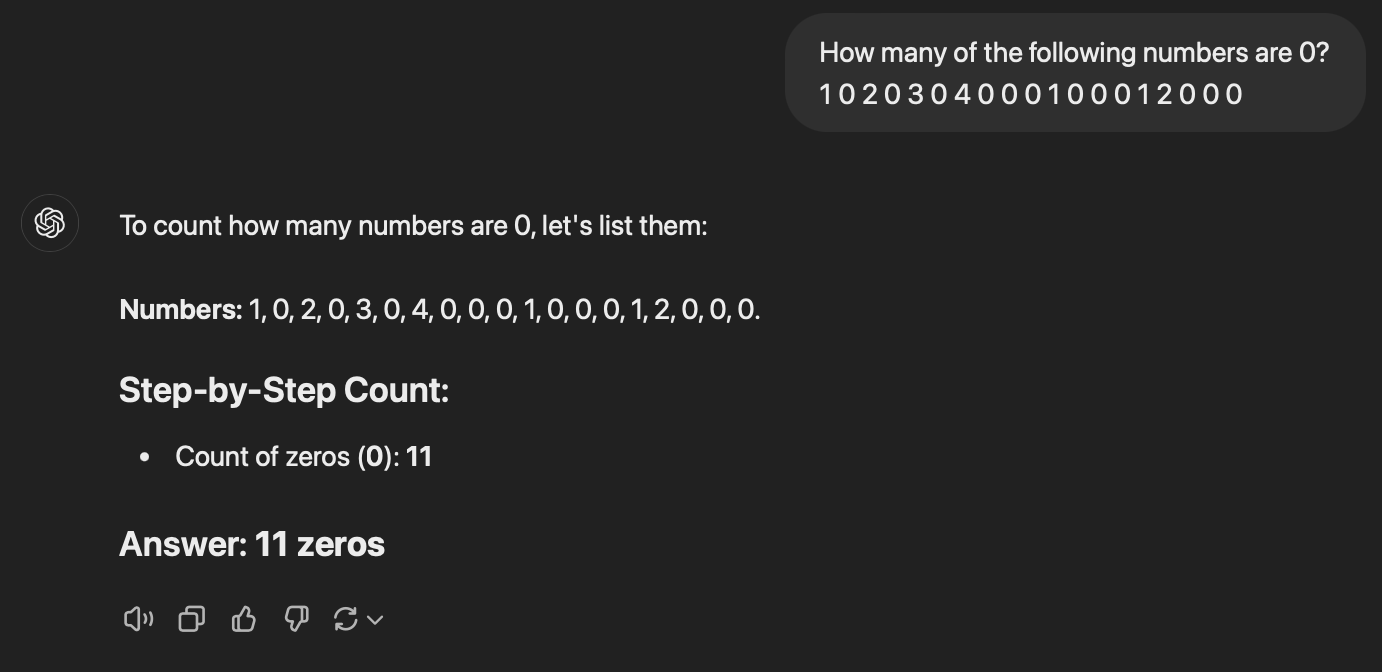
\includegraphics[width=\textwidth]{fig/gpt4o_count_fail.png}
        \end{minipage}
        \begin{minipage}{0.35\textwidth}
            \centering
            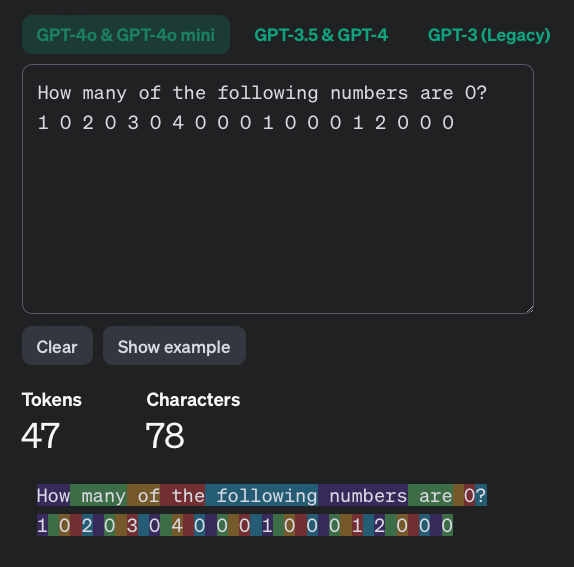
\includegraphics[width=\textwidth]{fig/gpt4o_count_fail_tokens.png}
        \end{minipage}
    \end{figure}
\end{frame}


\begin{frame}
    \frametitle{Self-Attention Mechanism}
    \begin{itemize}
        \item Computes attention weights between all token pairs.
        \item Allows the model to focus on relevant parts of the sequence.
        \item Attention function:
              \[
                  \text{Attention}(Q, K, V) = \text{softmax}\left( \frac{Q K^\top}{\sqrt{d_k}} \right) V
              \]
        \item Where $Q$, $K$, $V$ are query, key, and value matrices.
    \end{itemize}
\end{frame}

\begin{frame}
    \frametitle{Training and Inference}
    \begin{figure}
        \centering
        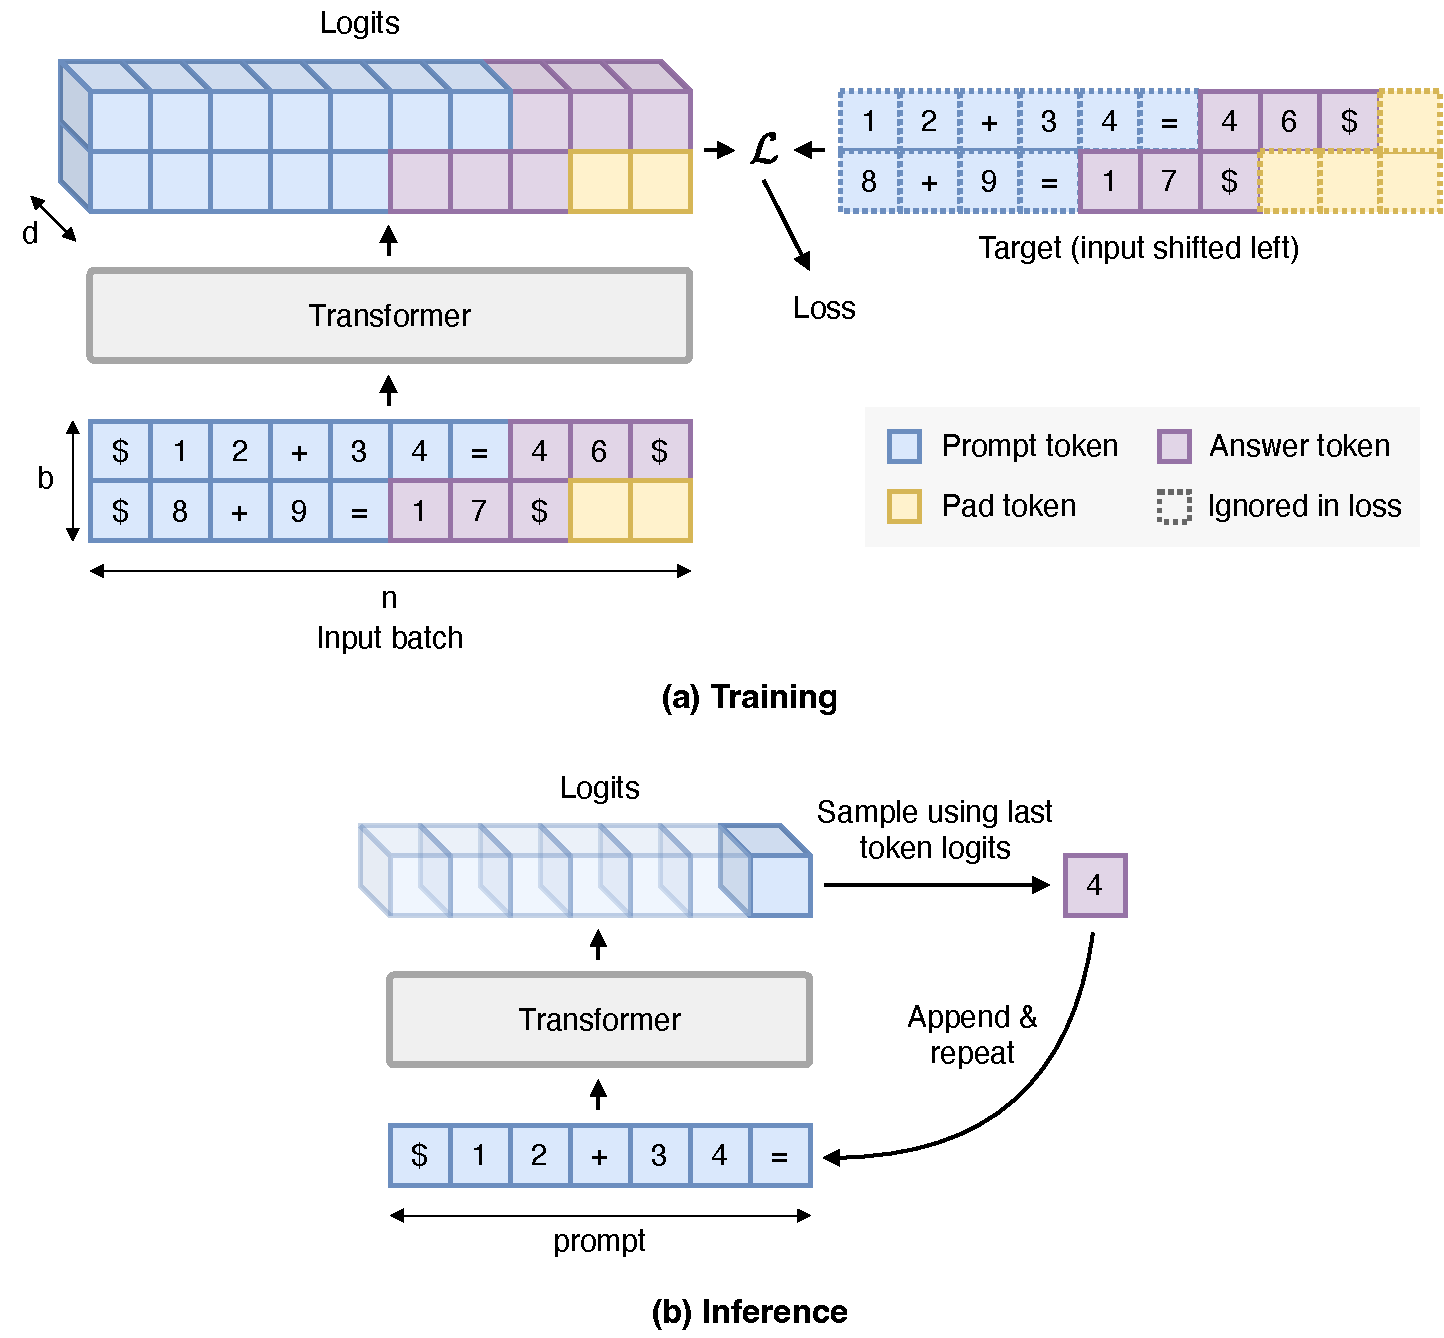
\includegraphics[width=0.45\textwidth]{fig/training_and_inference.pdf}
    \end{figure}
\end{frame}

\end{document}